\section{Resultate}

\subsection{Beobachtung}
\begin{frame}
	\begin{block}{Was beobachtet man bei Grenzfrequnez?}
		\begin{itemize}
			\item{$\varphi = 0$}
			\item{$\hat u_{Out} =$ maximal}
		\end{itemize}
	\end{block}
	\begin{exampleblock}{Warum ist das so?}
		\begin{itemize}
			\item Bei Resonanz wirkt die Schaltung rein resistiv.
			\item Ist etwas rein resistiv, kann es keine 
				Phasenverschiebung haben.
		\end{itemize}
	\end{exampleblock}
\end{frame}

\subsection{$f_0$ berechnet}
\begin{frame}
	\begin{block}{Werte beim berechneten Wert für $f_0$}
		\begin{itemize}
			\item $\varphi = 15^o$
			\item $\hat u_{Out} \neq$ maximal
		\end{itemize}
	\end{block}
	\begin{alertblock}{Warum ist das so?}
		\begin{itemize}
			\item Bauteile sind nur auf Papier ideal!
			\item Aufbau von Schaltungen (Layout) hat parasitäre
				Eigenschaften (abzuschätzen nach Grössenordnung)
		\end{itemize}
	\end{alertblock}
\end{frame}

\subsection{$f_0$ ermittelt}
\begin{frame}
	\begin{block}{Werte beim ermittelten Wert für $f_0$}
		\begin{itemize}
			\item $f_0 = 15.78kHz$
			\item $\hat u_{Out} =$ maximal
		\end{itemize}
	\end{block}
\end{frame}

\subsection{Sweap}
\begin{frame}
	\begin{columns}
		\begin{column}{5cm}
			\begin{block}{Sweep}
				Ein Sweep ist eine Wechselspannung 
				konstanter mit Amplitude, deren Frequenz 
				periodisch und stetig einen vorgegebenen 
				Bereich durchläuft. (Wikipedia)
			\end{block}
			\begin{exampleblock}{Was zeigt uns das?}
				Oberhalb und unterhalb von $f_0$ sinkt die
				Amplitude von $u_a$.
			\end{exampleblock}
		\end{column}
		\begin{column}{5cm}
			\begin{figure}
				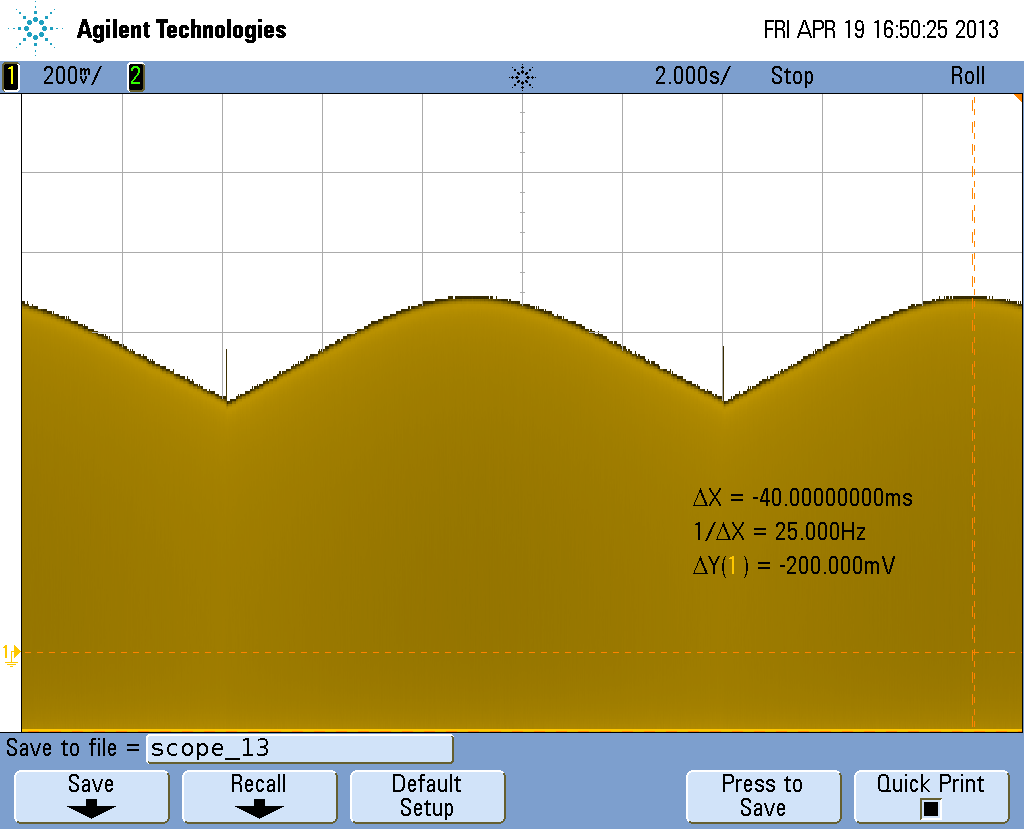
\includegraphics[width=0.95\textwidth]{scope_13.png}
				\caption{Sweep-Aufzeichnung}
			\end{figure}
		\end{column}
	\end{columns}
\end{frame}
